% !TeX root = ../slides.tex
\title{CS4221/CS5421}

\subtitle{Tutorial 8: XQuery and XSLT}

\author{Mark Meng Huasong}

\institute[National University of Singapore] % (optional, but mostly needed)
{
	School of Computing\\
	National University of Singapore
}

\titlegraphic{
	
\includegraphics[width=2cm]{nus-logo}
}

\date{Week 10, 2022 Spring}


\begin{frame}
	\titlepage
	\begin{tcolorbox}
		\begin{center}
			{\scriptsize \textcolor{red}{All the materials within presentation slides are protected by copyrights.\\
					It is forbidden by NUS to upload these materials to the Internet.}}
		\end{center}
	\end{tcolorbox}
\end{frame}

\begin{frame}[fragile]{An overview}
We have covered XML (data insertion), DTD and XPath in the last week.\\\vspace{10pt}
This week's tutorial covers XQuery and XSLT (e\underline{X}tensible \underline{S}tylesheet \underline{L}anguage \underline{T}ransformations).\\\vspace{10pt}
\begin{figure}
	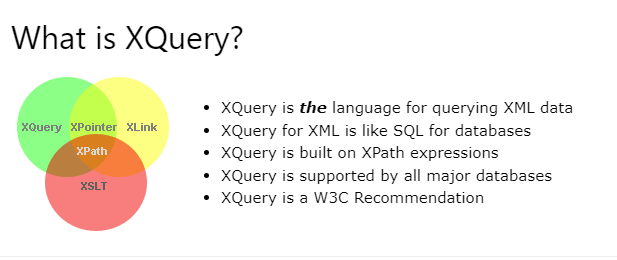
\includegraphics[width=0.75\textwidth,frame]{4221-t8/what.png}
	\caption{Picture cited from W3 School  \url{https://www.w3schools.com/xml/xquery_intro.asp}}
\end{figure}\vspace{-10pt}
\end{frame}

\section*{Section 1 XQuery}

\begin{frame}[fragile]{Question 1.1 (FLWOR Expression)}
A breif intro:\\\vspace{10pt}
(F) \textbf{for} + (L) \textbf{let} + (W) \textbf{where} + (O) \textbf{order by} + (R) \textbf{return} = FLWOR\\\vspace{10pt}

\begin{lstlisting}[style=xml-small-nomargin]
for $loop_var in doc("library.xml")/child::library/...
	let $var := $loop_var/child::.../text()
	let $var_2 := count($loop_var/child::...)
	...
	where $var [eq, ne, lt, le, gt, be, =, !=, <, >, <=, >=] {const}
	...
	order by $var [ascending, descending]
	return 
		{XML_expression_with_$var}
\end{lstlisting}

\begin{block}{XQuery Syntax for Where Clause}
	For the difference of general comparisons (e.g., =, <=, and etc) and value comparisons (e.g., eq, le, and etc), you may go to W3 School tutorial to read more details. \\
	\url{https://www.w3schools.com/xml/xquery_syntax.asp}
\end{block}
\end{frame}

\begin{frame}[fragile]{Question 1.1 Cont.}
Find the albums where the number of songs is greater than or equal to 3. Return the album title and count sorted by the count with the highest count appearing first. Your query should be written in the form of a FLWOR expression.\\\vspace{10pt}

For reference, your XML output should look somewhat similar to this:\\

\begin{lstlisting}[style=xml-small-nomargin]
<albums>
	<album>
		<title>No War</title>
		<count>4</count>
	</album>
	<album>
		<title>Bua Hati</title>
		<count>3</count>
	</album>
	<album>
		<title>Separuh Jiwaku Pergi</title>
		<count>3</count>
	</album>
</albums>
\end{lstlisting}
\end{frame}

\begin{frame}[fragile]{Question 1.1 Cont.}

\textbf{Solution:}
\begin{lstlisting}[style=xml-small]
<albums>{
	for $album in doc("library.xml")/child::library/child::album
		let $title := $album/child::title/text()
		let $count := count($album/child::songs/child::song)
		where $count ge 3
		order by $count descending
		return
			<album>
				<title>{$title}</title>
				<count>{$count}</count>
			</album>
}</albums>
\end{lstlisting}
\end{frame}

\begin{frame}[fragile]{Question 1.1 Cont.}
	
There is an alternative of writing XML expression in element-wise manner\\\vspace{5pt}

\textbf{Native XML approach}:
\begin{lstlisting}[style=xml-small-nomargin]
<album>
	for $album in doc("library.xml")/child::library/child::album
	...
	return
		<album>
			<title>{$title}</title>
			<count>{$count}</count>
		</album>
}</albums>
\end{lstlisting}


\textbf{Element-wise approach} (out-of-scope and not recommended).:
\begin{lstlisting}[style=xml-small-nomargin]
<album>
	for $album in doc("library.xml")/child::library/child::album
	...
	return
		element album{
			element title {$title},
			element count {$count}
		}
}</albums>
\end{lstlisting}

\end{frame}

\begin{frame}[fragile]{Question 1.2 (FLWOR Expression with Local Functions)}
	
Show the title and duration of the songs made by Indonesian artists sorted by duration in descending order. \\\vspace{5pt}
You may find declaring a local helper function as well as the built-in \texttt{tokenize(\$input, \$pattern)} function useful. For reference, your output should look something like this:\\\vspace{5pt}
\begin{columns}
\column{0.5\textwidth}
\begin{lstlisting}[style=xml-small-nomargin]
<songs>
	<song>
		<title>Miliki Diriku</title>
		<duration>10:35</duration>
	</song>
	<song>
		<title>Belajarlah Untuk Cinta</title>
		<duration>10:23</duration>
	</song>
	<song>
		<title>Bua Hati</title>
		<duration>5:35</duration>
	</song>
...
\end{lstlisting}
\column{0.47\textwidth}
\begin{lstlisting}[style=xml-small-nomargin]
...	
	<song>
		<title>Timang-Timang</title>
		<duration>5:13</duration>
	</song>
	<song>
		<title>Separuh Jiwaku Pergi</title>
		<duration>5:00</duration>
	</song>
	<song>
		<title>Hujanpun Menangis</title>
		<duration>4:17</duration>
	</song>
</songs>
\end{lstlisting}
\end{columns}
\end{frame}

\begin{frame}[fragile]{Question 1.2 Cont.}

The definition of a local function is like:	
\begin{lstlisting}[style=xml-small-nomargin]
declare function local:function_name($param_var as param_type) as return_type {
	let $local_var := ...
	return ...
};
\end{lstlisting}

\textbf{Reference of XQuery Types}: \url{https://docs.oracle.com/cd/E13214_01/wli/docs92/xref/xqtypecon.html}.\\
(e.g., xs:sting, xs:integer, xs:float, xs:double, xs:boolean, and etc)\vspace{10pt}

\textbf{Solution:} Start by declaring a function to get the duration as the number of seconds with type integer:\\\vspace{5pt}
\begin{lstlisting}[style=xml-small]
declare function local:duration-in-sec($duration-str as xs:string) as xs:int {
	let $min-secs := tokenize($duration-str, ':')
	return 60 * xs:int($min-secs[1]) + xs:int($min-secs[2])
};
\end{lstlisting}

\end{frame}

\begin{frame}[fragile]{Question 1.2 Cont.}
Let's write the XQuery statement in FLWOR format.\\\vspace{5pt}

Option 1: with \textbf{let}-binding\\\vspace{5pt}
\begin{lstlisting}[style=xml-small]
<songs>{
	for $song in doc("library.xml")/child::library/child::album[child::artists/child::artist/
		child::country = 'Indonesia']/child::songs/child::song
		let $duration := local:duration-in-sec($song/child::duration)
		order by $duration descending
		return $song
}</songs>
\end{lstlisting}

Option 2: without \textbf{let}-binding\\\vspace{5pt}
\begin{lstlisting}[style=xml-small]
<songs>{
	for $song in doc("library.xml")/child::library/child::album[child::artists/child::artist/
		child::country = 'Indonesia']/child::songs/child::song
		order by local:duration-in-sec($song/child::duration) descending
		return $song
}</songs>
\end{lstlisting}

\end{frame}

\begin{frame}[fragile]{Question 1.3 (Nested FLWOR)}
Show the list of titles of the albums made by Indonesian artists sorted by title. For each album show the songs sorted by duration in descending order.\\\vspace{5pt}
For reference, your HTML output when rendered should look somewhat similar to this: \\\vspace{-5pt}
\begin{columns}
\column{0.4\textwidth}
\begin{figure}
	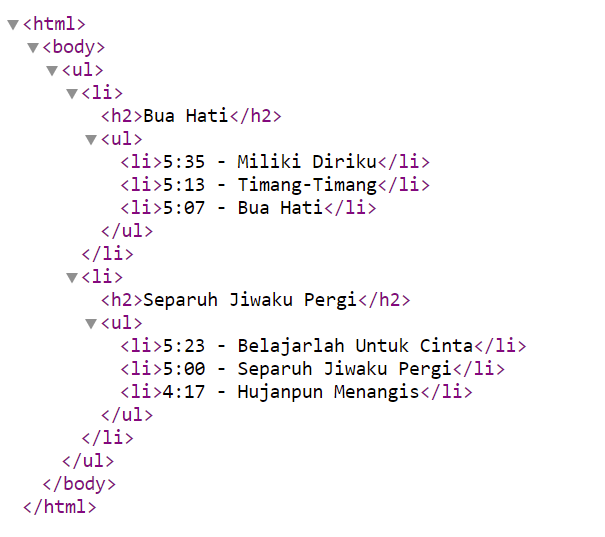
\includegraphics[width=1\textwidth,frame]{4221-t8/q3-output.png}
\end{figure}\vspace{-5pt}
(HTML code view)
\column{0.35\textwidth}
\begin{figure}
	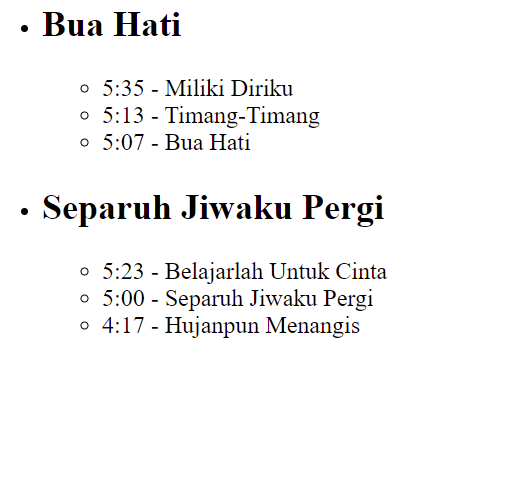
\includegraphics[width=1\textwidth,frame]{4221-t8/q3-output-direct.png}
\end{figure}\vspace{-5pt}
(Direct output (as shown in eXide))
\end{columns}
\end{frame}

\begin{frame}[fragile]{Question 1.3 Cont.}

First of all, let's construct a draft. \\
\begin{lstlisting}[style=xml-small]
<html>
	<body>
		<ul>{
			<!-- We only want albums made by Indonesian artists -->
			for $album in doc("library.xml")//album[artist/country = 'Indonesia']
				let $album-title := $album/title/text()
				order by $album-title
				return
					<li>
					<!-- For each album we want to output all songs titles and duration, sorted by their duration in descending order -->
					<h2>{$album-title}</h2>
					<ul>{
						for $song in $album//song
						order by local:duration-in-sec($song/duration) descending
						return
						<li>{$song/duration/text()} - {$song/title/text()}</li>
					}</ul>
					</li>
		}</ul>
	</body>
</html>
\end{lstlisting}


\end{frame}

\begin{frame}[fragile]{Question 1.3 Cont.}
	
\textbf{Solution}: (Always use complete writing with ``\textbf{child::}'' in the exam/test.)\\
\begin{lstlisting}[style=xml-small-nomargin]
declare function local:duration-in-sec($duration-str as xs:string) as xs:int {
		let $min-secs := tokenize($duration-str, ':')
		return 60 * xs:int($min-secs[1]) + xs:int($min-secs[2])
};
<html>
	<body>
		<ul>{
			for $album in doc("library.xml")/child::library/child::album[child::artists/child::artist/child::country = 'Indonesia']
				let $album-title := $album/child::title/text()
				order by $album-title
				return
					<li>
						<h2>{$album-title}</h2>
						<ul>{
							for $song in $album/child::songs/child::song
								order by local:duration-in-sec($song/child::duration) descending
							return
								<li>{$song/child::duration/text()} - $song/child::title/text()}</li>
						}</ul>
					</li>
		}</ul>
	</body>
</html>
\end{lstlisting}
	
	
\end{frame}

\begin{frame}[fragile]{Question 1.4 (XQuery with Styled Output)}
Color the songs with a duration greater than or equal to \textcolor{red}{\cancel{600}} \textbf{300} seconds green and otherwise red.\\\vspace{5pt}
Note that ``||'' is used in XQuery for string concatenation. For reference, your HTML output when rendered should look somewhat similar to this: \\\vspace{0pt}

\begin{columns}
	\column{0.5\textwidth}
	\begin{figure}
		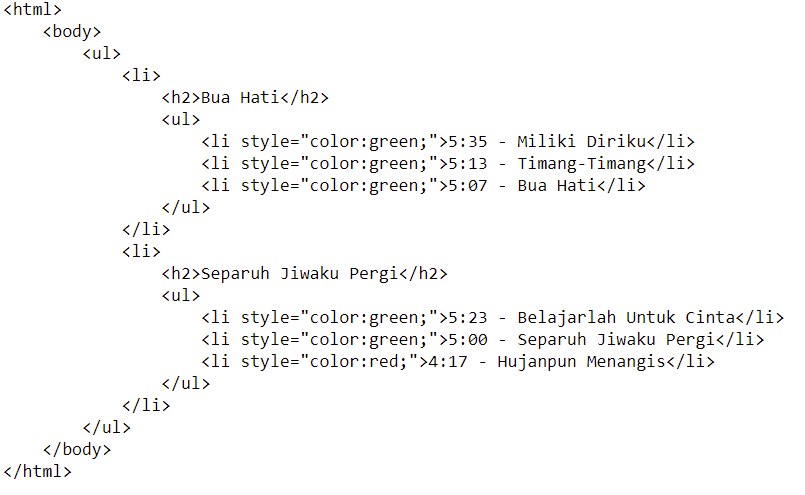
\includegraphics[width=1\textwidth,frame]{4221-t8/q4-output.png}
	\end{figure}\vspace{-5pt}
	(HTML code view)
	\column{0.35\textwidth}
	\begin{figure}
		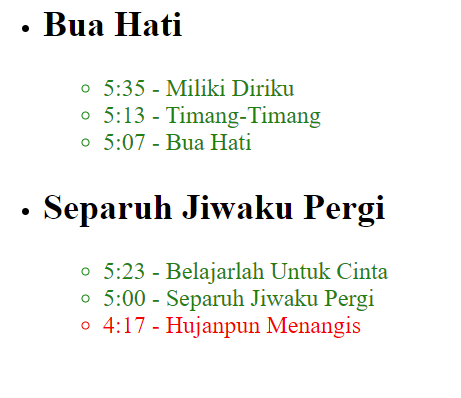
\includegraphics[width=1\textwidth,frame]{4221-t8/q4-output-direct.png}
	\end{figure}\vspace{-5pt}
	(Direct output)
\end{columns}
\vspace{5pt}
\textbf{Solution shown in the next slide.}
\end{frame}
	
\begin{frame}[fragile]{Question 1.4 Cont.}
\vspace{-5pt}
\begin{lstlisting}[style=xml-small]
<!-- We keep the function local:duration-in-sec unchanged --><!-- omitted -->
<html>
	<body>
		<ul>{
			for $album in doc("library.xml")/child::library/child::album[child::artists/child::artist/child::country = 'Indonesia']
				let $album-title := $album/child::title/text()
				order by $album-title
				return
				<li>
				<h2>{$album-title}</h2>
				<ul>{
					for $song in $album/child::songs/child::song
						let $duration := local:duration-in-sec($song/child::duration)
						let $li-color := (if ($duration >= 300) then 'green' else 'red')
						order by $duration descending
						return
							<li style="color:{$li-color};">
								{$song/child::duration/text()} - {$song/child::title/text()}
							</li>
				}</ul>
				</li>
		}</ul>
	</body>
</html>
\end{lstlisting}\vspace{5pt}
\end{frame}

\begin{frame}[fragile]{Question 1.4 Cont.}
You can also get rid of let clause (\$li\_color) by defining color in the return:\\
\begin{lstlisting}[style=xml-small-nomargin]
...
return
	<li style="color:{(if ($duration >= 300) then 'green' else 'red')};"> 
		{$song/child::duration/text()} - {$song/child::title/text()}
	</li>
\end{lstlisting}
	
The element-wise approach alternative can be written as:\\
\begin{lstlisting}[style=xml-small-nomargin]
...
return
	element li {
		attribute style {
			if ($duration >= 600) then 'color:green;' else 'color:red;'
		},
		$song/child::duration/text() || ' - ' || $song/child::title/text()
	}
\end{lstlisting}
	
\end{frame}
	
\begin{frame}[fragile]{Question 1.5}
Find the albums where the total listening duration (the sum of all the album's songs' duration) is greater than 1100 seconds. The albums should be sorted by title. In the XML output, you should return the album elements that satisfy the constraint with the title and an extra attribute duration. Your main code should be formed as a FLWOR expression. You may use functions you have declared in previous questions.\\\vspace{5pt}
For reference, your XML output should look somewhat similar to this:\\\vspace{5pt}

\begin{lstlisting}[style=xml-small-nomargin]
<albums>
	<album>
		<title>Bua Hati</title>
		<duration>1283</duration>
	</album>
	<album>
		<title>Separuh Jiwaku Pergi</title>
		<duration>1180</duration>
	</album>
</albums>
\end{lstlisting}\vspace{5pt}	
\end{frame}

\begin{frame}[fragile]{Question 1.5 Cont.}
\textbf{Solution}: \\
\begin{lstlisting}[style=xml-small-nomargin]
<!-- We keep the function local:duration-in-sec unchanged -->
<albums>{
	for $album in doc("library.xml")/child::library/child::album
		let $title := $album/child::title/text()
		let $durations := $album/child::songs/child::song/child::duration
		let $total-duration := sum(for $duration in $durations return local:duration-in-sec($duration))
		where $total-duration gt 1100
		order by $title
		return
			<album>
				<title>{$title}</title>
				<duration>{$total-duration}</duration>
			</album>
}</albums>
\end{lstlisting}
\end{frame}


\begin{frame}[fragile]{Question 1.6}
Explain a key difference between the for loop used in XQuery compared to an imperative language such as Python.\\\vspace{10pt}

\textbf{Solution}: \\
XQuery is a functional language. Each iteration is executed in parallel and no communication between the threads are allowed. This is in contrast to imperative languages where the iterations are executed sequentially and may i.e. increment a counter or likewise. See XQuery/FLWOR Expression for more info.

\begin{block}{To read more...}
The XQuery Tutorial on W3 School: \url{https://www.w3schools.com/xml/xquery_intro.asp}
\end{block}	
\end{frame}

\section*{Section 2 XSLT}
\begin{frame}[fragile]{Question (XSL) 2.1}
Write an XSLT stylesheet that displays in a table or a list of an HTML document the name and released year of the albums with genre “Pop” of the XML document.\\\vspace{5pt}
Prefer XSLT template matching with ``\textbf{value-of}'' and ``\textbf{apply-template}'' to imperative control structures (e.g. ``\textbf{for-each}'').\\\vspace{10pt}

\end{frame}

\begin{frame}[fragile]{Question (XSL) 2.1 Cont.}
\textbf{Brief:}\\\vspace{10pt}
XSLT is another technique to make query.\\\vspace{5pt}
XSL is still a (special) XML file with its own syntax.\\ \vspace{5pt}
XSL can be used to \textbf{navigate}, \textbf{query} and \textbf{transform} the data in the XML library.\\\vspace{5pt}
XSLT describes the \textbf{transformation process} of a given XSL over the existing data. 
\end{frame}

\begin{frame}[fragile]{Question (XSL) 2.1 Cont.}
\textbf{Solution}: (Save the code below into an \textbf{.xsl} file)\\
\begin{lstlisting}[style=xml-small-nomargin]
<?xml version="1.0" encoding="UTF-8"?>
<xsl:stylesheet xmlns:xsl="http://www.w3.org/1999/XSL/Transform" version="1.0">
<!-- We generally always start with the root -->
<xsl:template match="/">
	<html>
		<body>
			<ul>
				<xsl:apply-templates select="child::library/child::album[child::genres/child::genre='Pop']"/>
			</ul>
		</body>
	</html>
</xsl:template>

<xsl:template match="album">
	<li>
		Album <xsl:value-of select="title"/> (<xsl:value-of select="year"/>)
	</li>
</xsl:template>

</xsl:stylesheet>
\end{lstlisting}\vspace{5pt}

\end{frame}

\begin{frame}[fragile]{Question 2.2 (Transformation)}
Perform XSLT transformation through eXist-db using the XSLT file you just created.\\\vspace{5pt}

\textbf{Solution}:

\begin{lstlisting}[style=xml-small-nomargin]
transform:transform(doc("library.xml"), doc("library.xsl"), ())
\end{lstlisting}\vspace{5pt}

We don't need parameters in XSLT for this module.

\begin{block}{To read more...}
	The XSLT Tutorial on W3 School: \url{https://www.w3schools.com/xml/xsl_intro.asp}
\end{block}	
\end{frame}


\begin{frame}[fragile]{To wrap-up: the big picture of XPath, XQuery and XSLT}
\begin{columns}

\column{0.25\textwidth}
\begin{figure}
	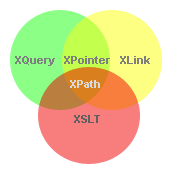
\includegraphics[width=1\textwidth]{4221-t8/what-small.png}
\end{figure}\vspace{5pt}

\column{0.73\textwidth}

\textbf{Can you implement the Question 2 in XQuery?}\\\vspace{5pt}
\begin{lstlisting}[style=xml-small-nomargin]
<html>
	<body>
	<ul>{
		for $album in doc("library.xml")//album[genres/genre = 'Pop']
		let $album-title := $album/title/text()
		let $album-year := $album/year/text()
		return
			<li> Album {$album-title} ({$album-year}) </li>
	}</ul>
	</body>
</html>
\end{lstlisting}
In fact, you can find the XQuery approach is simpler.
\end{columns}
\end{frame}

\begin{frame}[fragile]{More exercise}
	
\begin{block}{Optional}
Zemmy post a thread on the Luminus Forum for extra exercise on XQuery/XSLT. Feel free to have a try.
\end{block}

\end{frame}

\begin{frame}{}
	\centering  
	For any further question, please feel free to email me:\vspace{10pt}
	
	huasong.meng@u.nus.edu \vspace{20pt}
	
	\begin{tcolorbox}
		\begin{center}
			\textcolor{red}{Copyright 2021 Mark H. Meng. All rights reserved.}
		\end{center}
	\end{tcolorbox}
\end{frame}